\documentclass{sig-alternate}
\usepackage{amsmath,amssymb}
\usepackage{graphicx}
\usepackage{hyperref}

\begin{document}
\title{DBCC: Compiling Databases for High-Performance View Maintenance and Update Stream Processing}
\numberofauthors{2}
\author{
\alignauthor Yanif Ahmad\\
    \affaddr{Computer Science Dept.}\\
    \affaddr{Cornell University}\\
    \email{yanif@cs.cornell.edu}
\alignauthor Christoph Koch\\
    \affaddr{Computer Science Dept.}\\
    \affaddr{Cornell University}\\
    \email{koch@cs.cornell.edu}
}
\maketitle

\section{Introduction}

\section{System Overview}

\begin{itemize}
\item Application embedded vs. server cluster processing models
\item Brief architecture description for each mode.
\item Role of the compiler in the architecture.
\end{itemize}

\section{Recursive Compilation}
\def\algsum{\mathrm{sum}}

\subsection{Map Algebra}
Describe:
\begin{itemize}
\item map algebra grammar, and define terms, including variables,
  constraints for unifications, and domains. 
\item simplifications for presentation, i.e. assuming single top-level
  algebra, although we can easily extend to handle sums/products of top-level
  aggregates.
\item relationship of group-by to a top-level map with dimensionality
  given by group-by attributes, as opposed to a top-level nullary map for simple
  aggregate queries.
\item compilation overview, i.e. two primary phases delta pushdown and
  aggregate simplification.
\end{itemize}

\subsection{Query Compilation}

\subsubsection{Delta Query Derivation}
Describe:
\begin{itemize}
\item concept of delta pushdown, and present delta rules.
\item delta rule for predicates and the fact that in general, we do not
  have positive relational algebra for insertions due to the fact that with
  using the results of nested aggregate queries in predicates, tuples can be
  both added and removed from the result set of the predicate. Refer to possible
  optimizations of this rule, e.g. monotonic case.
\end{itemize}

\subsubsection{Aggregate Simplification}
Describe/define:
\begin{itemize}
\item semiring abstraction of map and relational algebra.
\item polynomials of map and relational algebra, and discuss
canonicalization of queries to polynomials (i.e., $roly\_poly$). Discuss
potential exponential blowup of terms, but this allows full separation of delta
terms from old values.
\item factorization of monomials (i.e. join trees), enabling distribution
  of aggregates over joins, to join inputs. Describe factorization as performed
  by finding connected components on a attribute-usage graph.
\end{itemize}

\subsubsection{Domain Maintenance}
Describe:
\begin{itemize}
\item need to compute the value of a nested query when presented with
  an outer variable value that has not been seen, and the subsequent insertion
  into the map key domain.
\item simple implementation with naive compilation, that can be
  optimized when certain properties hold over the nested query. Refer to section
  on monotonic nested queries below.
\item reclamation of values in then map key domain when the nested
  query value returns to its initial implicit state.
\end{itemize}

\subsection{Compilation Examples}
\subsubsection{Flat query compilation example}
\begin{itemize}
\item Example: $\algsum_{a*d}(R \bowtie S \bowtie T)$, using demo-style table,
  or a tree figure.
\end{itemize}

\subsubsection{Nested query compilation example}
\begin{itemize}
\item Example: VWAP query
\[\algsum_{p*v}(\sigma_{k*\algsum_{v1}(\rho_{p1,v1}(bids)) -
    \algsum_{v2}(\sigma_{p2 > p}(\rho_{p2,v2}(bids)))}(bids))\]
\end{itemize}

\subsection{Code Generation}
Describe:
\begin{itemize}
\item accumulator language which allows simple code generation for
procedural languages such as C++/Java.
\item differences between simple accumulator language and implementations of
relational algebra which pass around sets, resulting in a larger greater copying
of data and more memory pressure. Accumulator language is even different to
pipelining query plans, which can push tuples through to an accumulator
(i.e. incr() function of an aggregate) at a tuple granularity, but still copies
data from using an operator processing model.
\end{itemize}

\section{Compiler extensions}
\subsection{Min/Max aggregates}
\begin{itemize}
\item Aggregate rules for min/max queries.
\item Describe the need to maintain relational state for handling delete min/max.
\item Describe the issues with nesting min/max aggregates with existing map
  algebra terms.
\end{itemize}

\subsection{Monotonic nested queries}
\begin{itemize}
\item Describe potential to keep only a limited subset of variables defined from
  outer queries, which in the extreme case of monotonic queries simplifies down
  to a single value.
\item Describe data structures enabling initial values to be computed from
  the nested query result of a neighbouring outer variable value.
\end{itemize}

\subsection{Compiling multiple queries}
\begin{itemize}
\item Currently support multiple aggregates specified on top of the same
  relational statement, which may subsequently share maps if there are any
  equivalent map algebra expressions found common during compilation.
\item We partition queries with common (but not an equivalent set of) input
  relations into compilation units, enabling handler functions to be created for
  each compilation unit. This prevents monolithic event handlers, thus our
  compiled database engine may call multiple handlers for a single update stream.
\end{itemize}

\section{Experiments}
Experimental setup:
\begin{itemize}
\item DBToaster implemented in xxx lines of Ocaml code, currently not a
  multithreaded compiler.
\item dbksrv02 specs: xxx GHz Xeon Processor, 16Gb RAM.
\item Single OS setup for comparability: Linux. This means we can't use SQL
  Server, and should use Oracle instead.
\item Queries: TPCH, SSB, VWAP, MACD, Linear Road avg lav.
\item Datasets: TPCH generated, orderbook data from NASDAQ, and Linear Road
  generated from MITSIM.
\item DBToaster implementations for comparison points:
    \begin{itemize}
    \item Naive compilation: query-plan based compilation, with joins
      implemented as IL-joins or hash-joins. Note we will not implement a
      DP-optimizer, but simply manually specify join algorithm for our workload.
      This is intended to reflect existing (purely in-memory) implementations of
      query plans.
    \item Recursive compilation $RC(k)$: compilation that applies k- levels of
      recursive compilation.
    \item Incremental view maintenance: $RC(1)$.
    \item DBToaster: $RC(\infty)$.
    \end{itemize}
\end{itemize}

\subsection{Query Processing Performance}
\subsubsection{Synthetic workloads}
\begin{itemize}
\item Nested workload: simple linear nesting, with varying nesting levels $k=1..5$ i.e.
\[sum_{sum_{sum_{f}(Q_1)}(Q_2)}(Q_3)\]

\item Join workload: fixed set of join graphs, with varying \# relations
  $k=1..10$. Join graphs should include chains, and stars, and if time permits
  cycles simplified with hypergraph decomposition.

\item What dataset should we use here? TPCH/orderbook data, or generate
  synthetic distributions?

\item Notes on subquery processing in existing DBMS:
    \begin{itemize}
    \item Common techniques: subquery flattening, handling duplicates via a
    semijoin, replacing exists/any operators for single-row subqueries w/ early termination, etc.
    \item Apache Derby's subqueries:
    \url{http://db.apache.org/derby/docs/10.0/manuals/tuning/perf105.html#HDRSII-TRANSFORM-13699}
    \item Oracle's optimization of subqueries:
    \url{http://www.oracle.com/technology/products/bi/db/10g/pdf/twp_general_query_optimization_10gr2_0605.pdf}
    \item Oracle includes several implementations of semijoins, (hash-, sort-merge,
    etc.) allowing join optimization just as with regular joins.
    \item SQL Server subquery types:
    \url{http://technet.microsoft.com/en-us/library/ms175838.aspx}
    \item How does our naive nesting implementation compare with other DBMS's
    implementations of semijoins?
        \begin{itemize}
        \item We can ignore in/exists/any/all subqueries, and focus on scalar subqueries in predicates
        and select lists.
        \item Scalar aggregate subqueries must be evaluated fully, however, the subquery results for
        duplicate outer attributes can be cached and reused.
        \end{itemize}
    \end{itemize}

\item Predicted running times:
    \begin{itemize}
    \item Indexed $k$-way nested loops joins w/ accumulators: $O(n\log^{k-1}{n})$
    \item RC(k): $\sum_{m \in maps(k)} {\mbox{update cost}(m)}$
    \end{itemize}
\end{itemize}

\begin{figure}
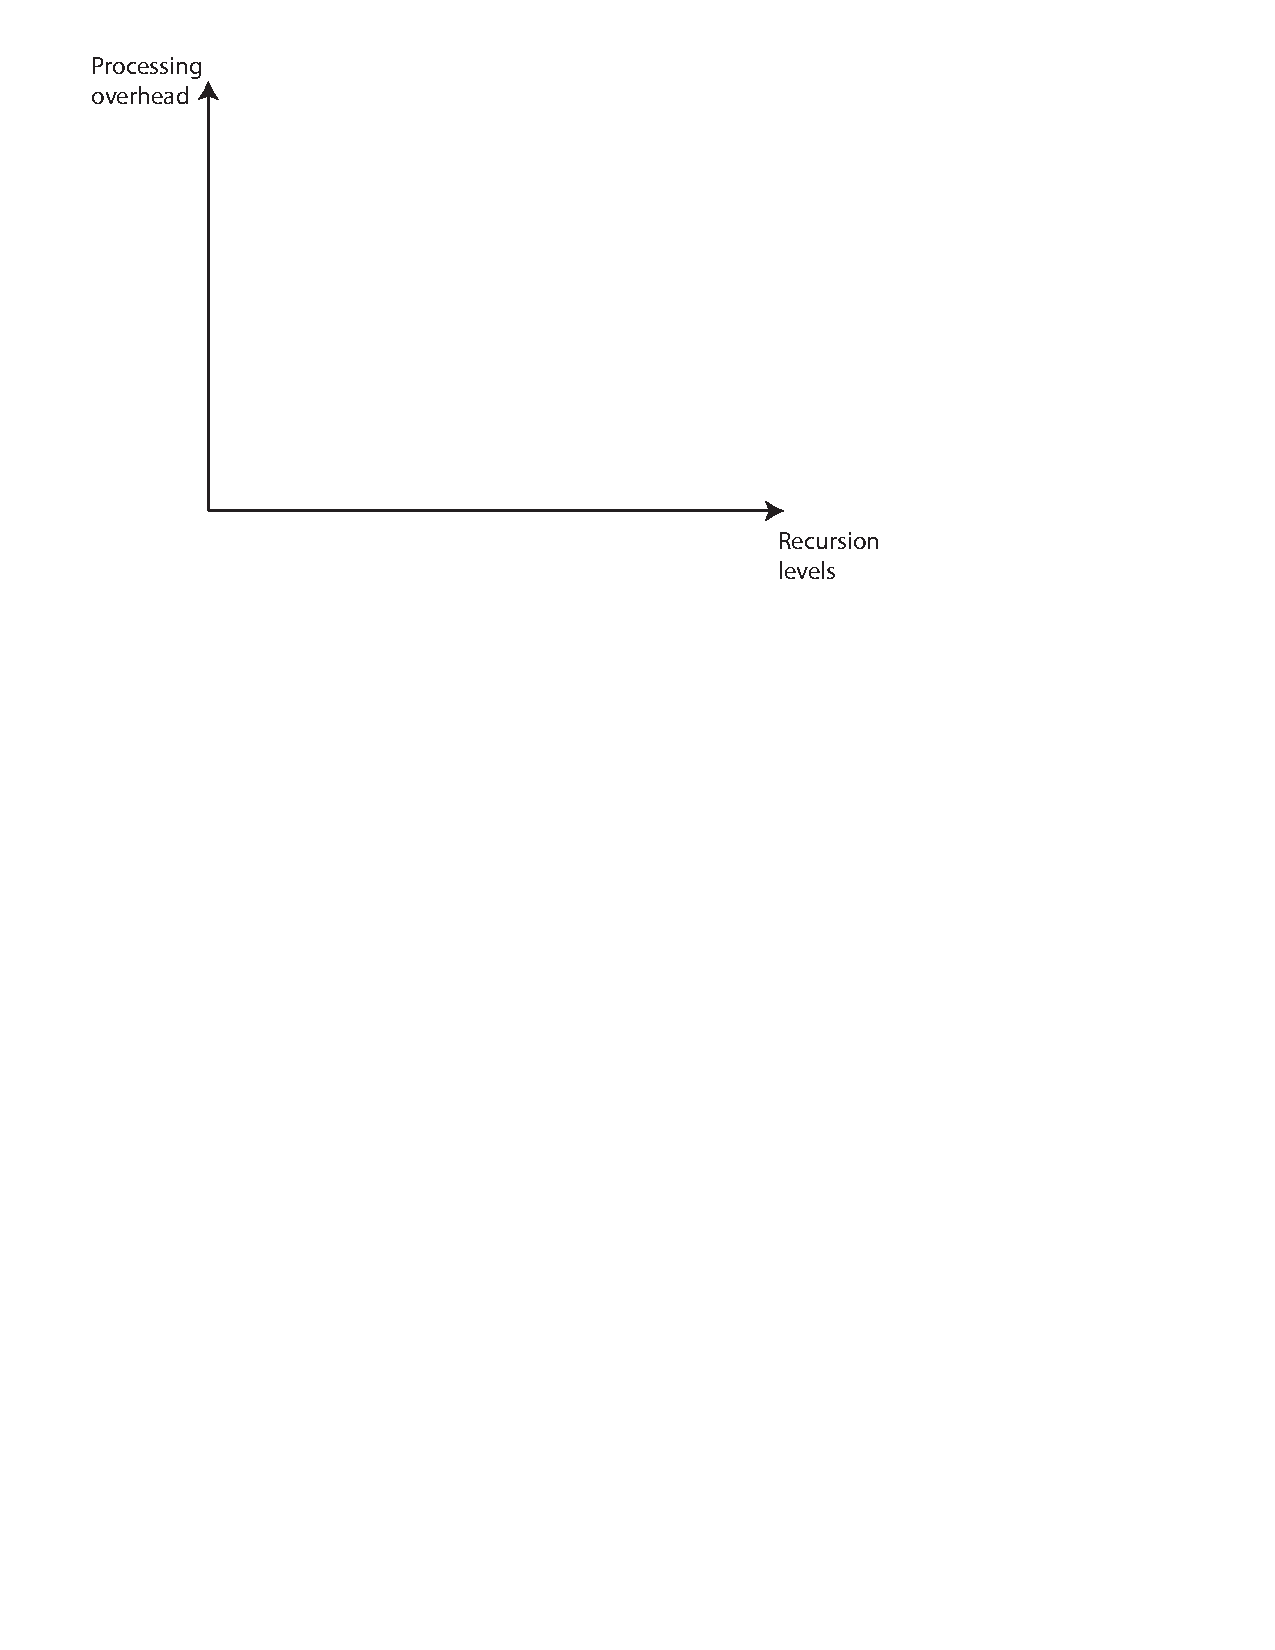
\includegraphics[scale=0.6]{figures/axes-rlevels.pdf}
\caption{Query processing overhead under varying degrees of recursive
compilation aggressiveness, for a \textit{k}-nested query.}
\label{fig:overhead-recursion-levels-nesting}
\end{figure}

\begin{figure}
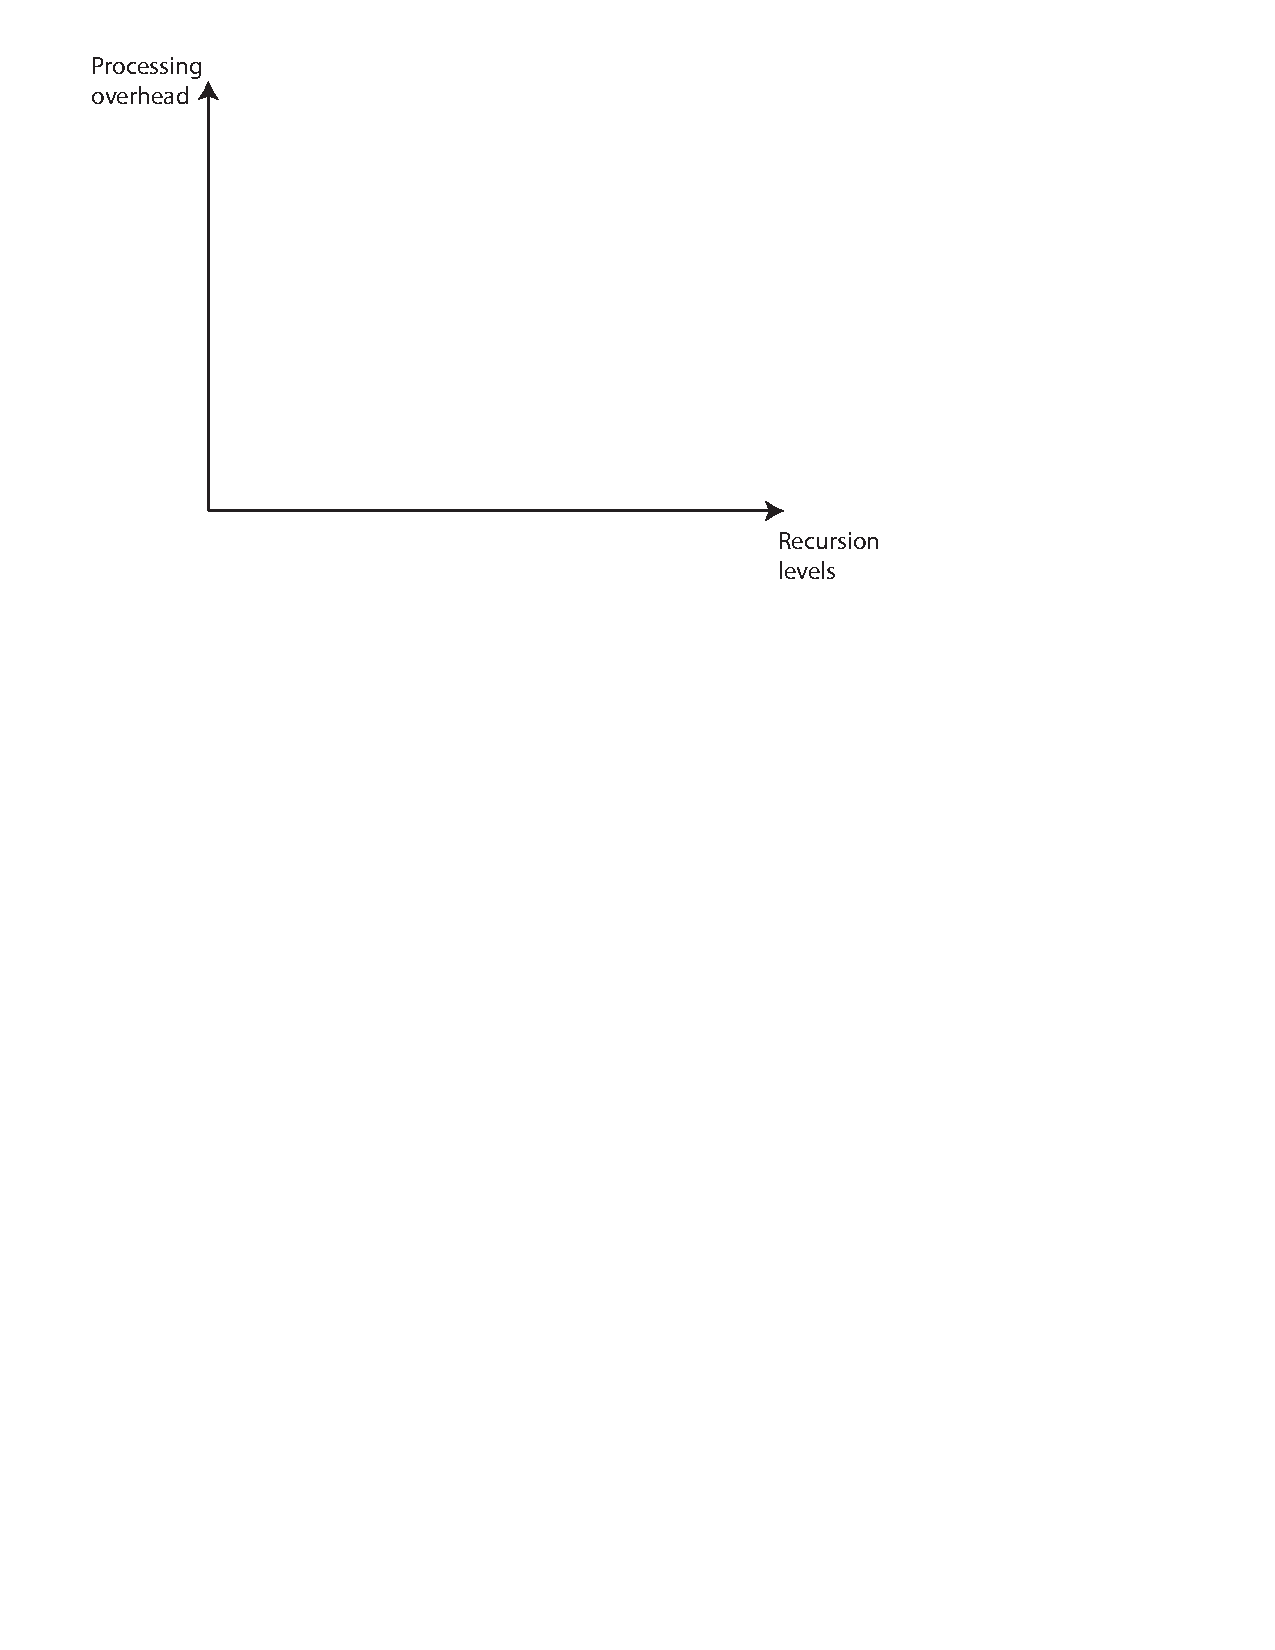
\includegraphics[scale=0.6]{figures/axes-rlevels.pdf}
\caption{Query processing overhead under varying degrees of recursive
compilation aggressiveness, for a \textit{k}-way join.}
\label{fig:overhead-recursion-levels-join}
\end{figure}

\begin{figure}
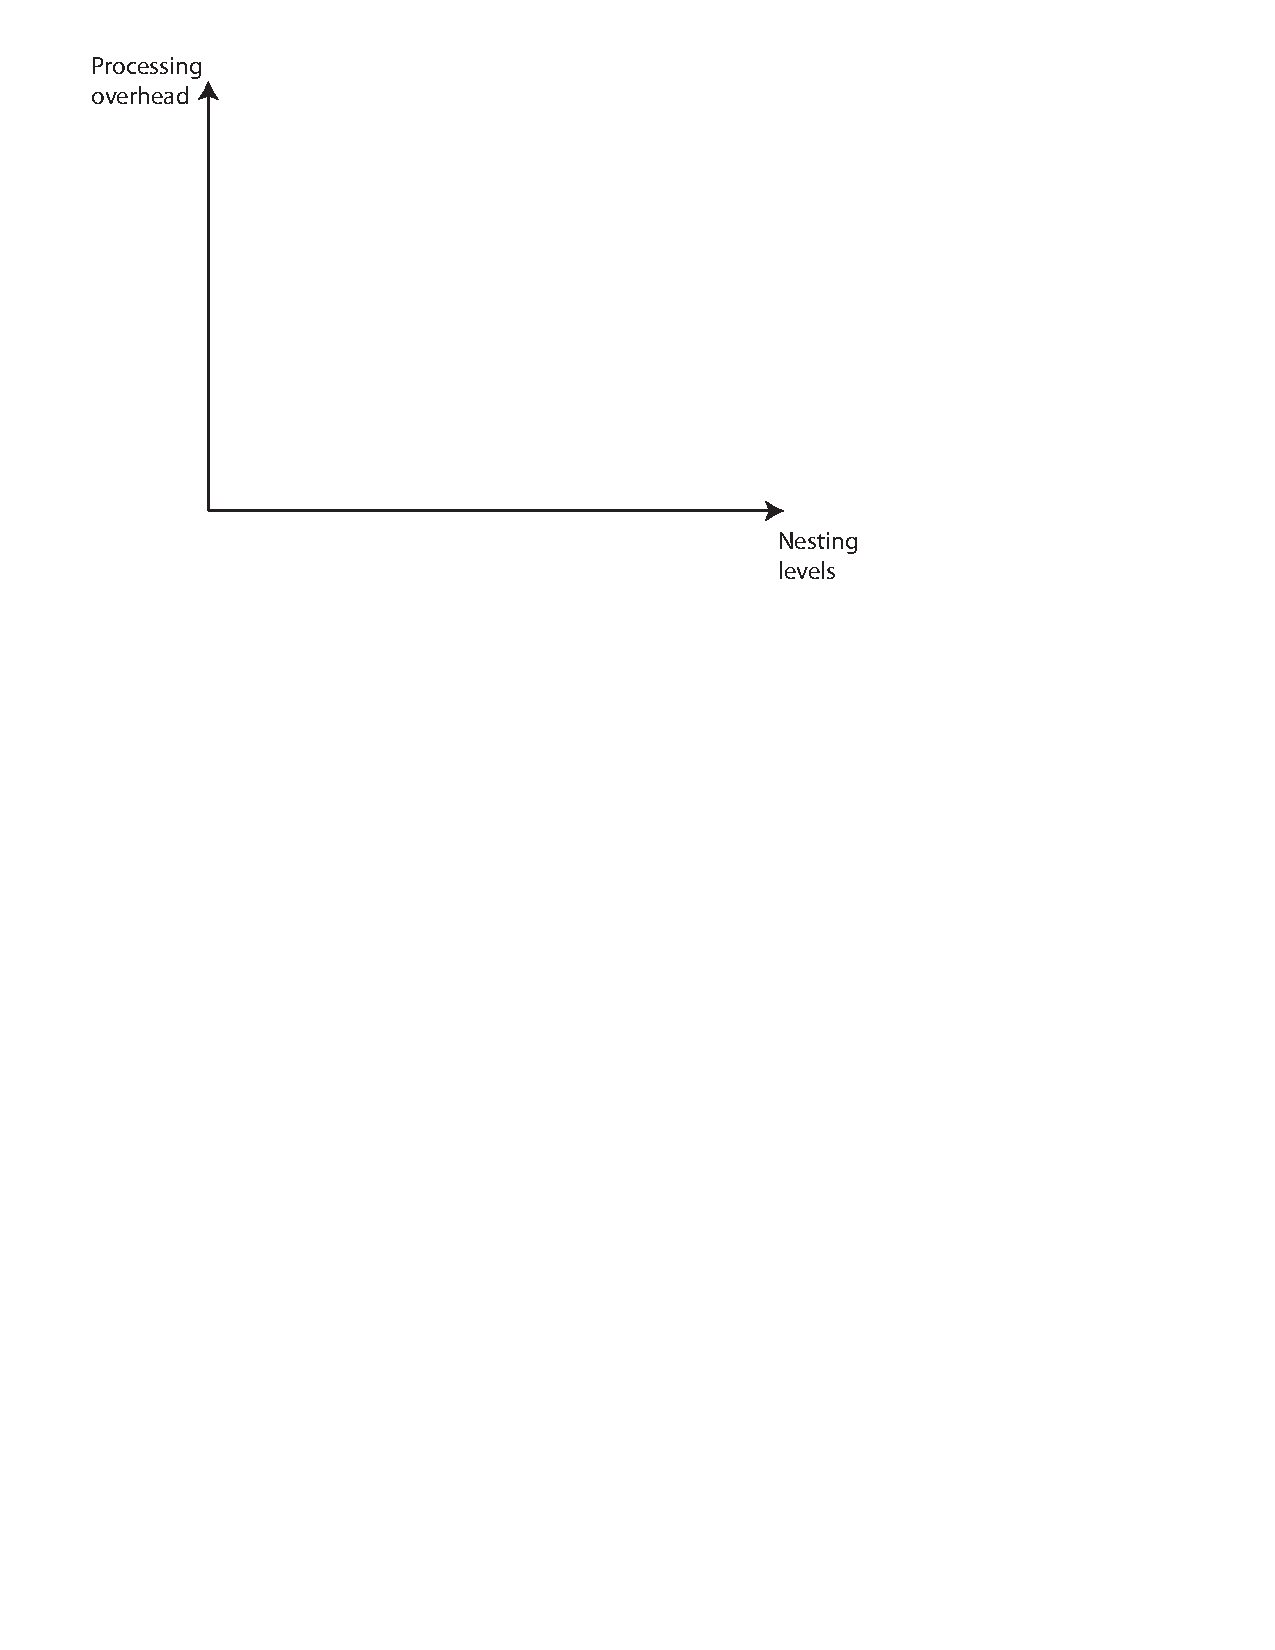
\includegraphics[scale=0.6]{figures/axes-nlevels.pdf}
\caption{Query processing overhead under varying nesting workloads, for
recursive compilation and incremental view maintenance.}
\label{fig:overhead-workload-nesting}
\end{figure}

\begin{figure}
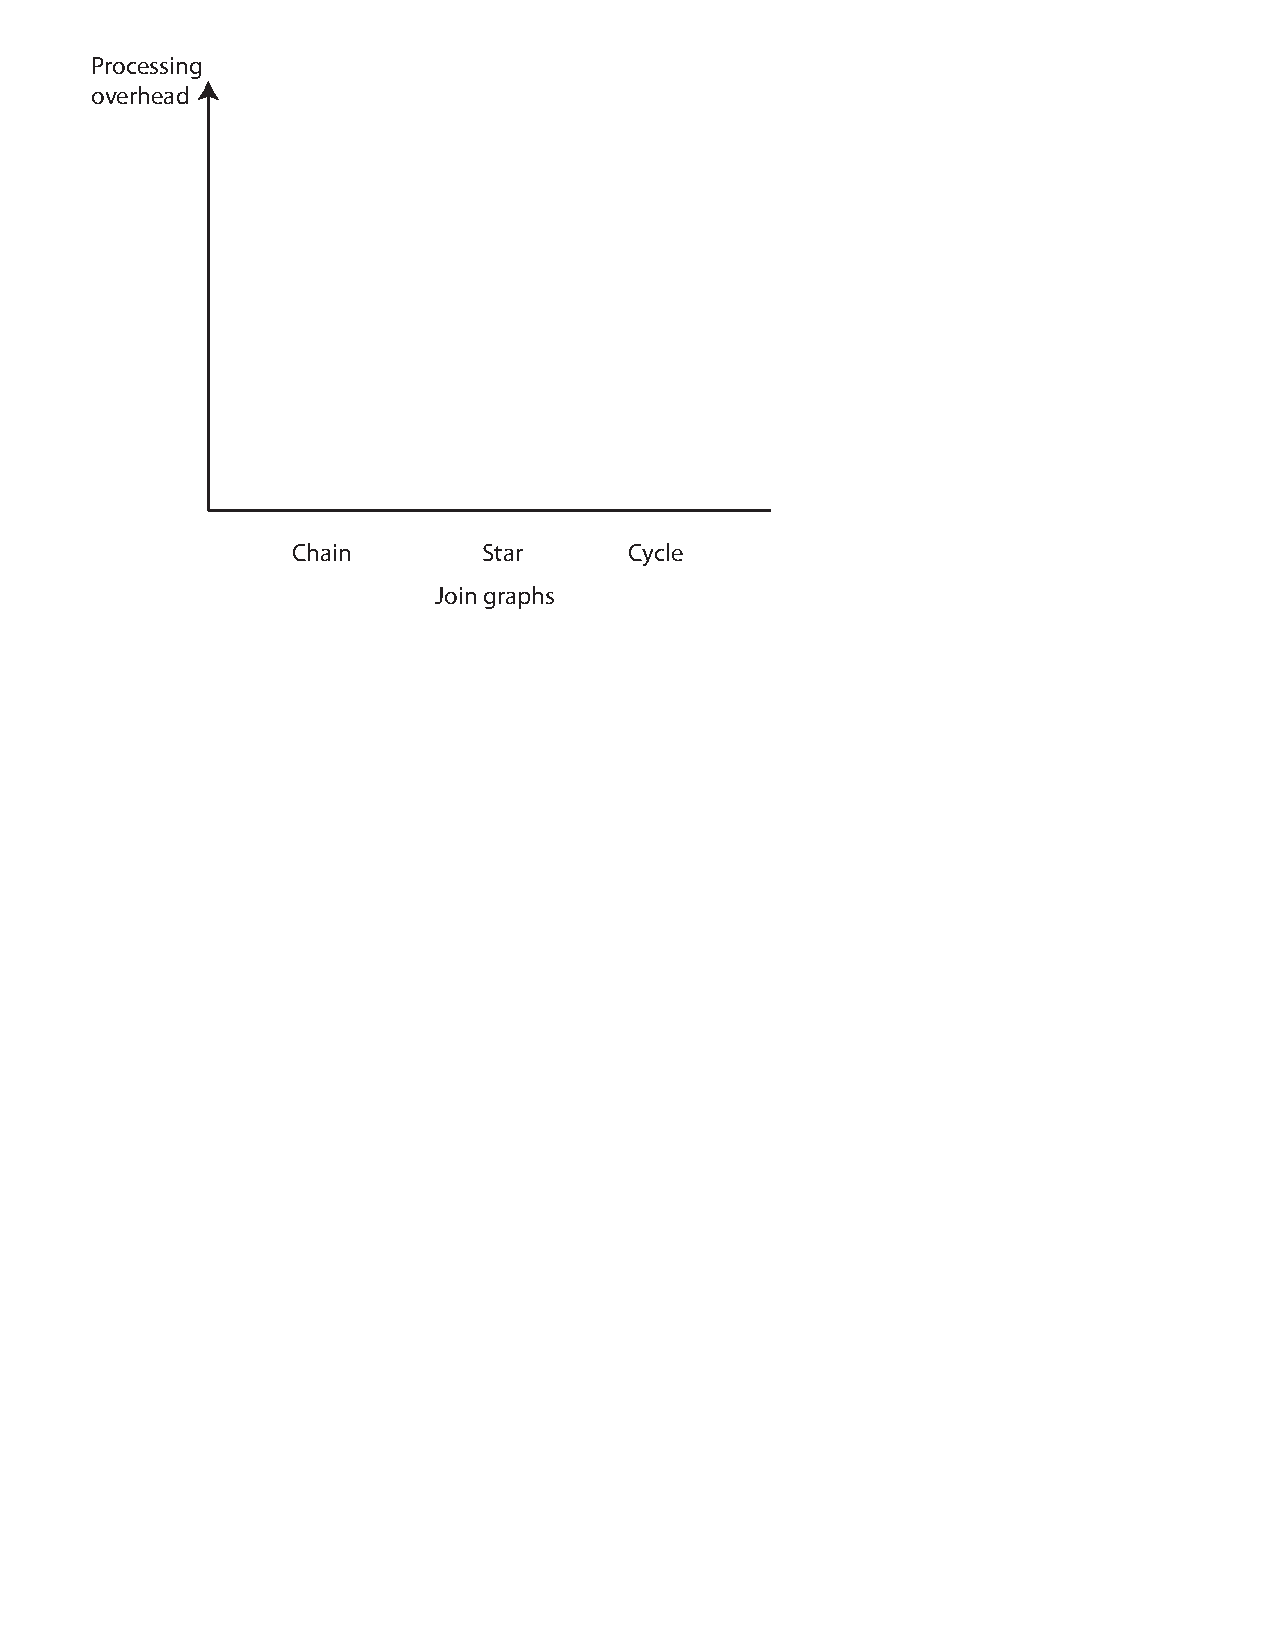
\includegraphics[scale=0.6]{figures/axes-jgraph.pdf}
\caption{Query processing overhead under varying join graph workloads for
recursive compilation and incremental view maintenance.}
\label{fig:overhead-workload-join}
\end{figure}

\subsubsection{Algorithmic Trading and Data Warehousing applications}
\begin{itemize}
\item Compare naive query processing and incremental view maintenance to full
DBToaster recursive compilation for real-world scenarios.
\end{itemize}

\begin{figure}
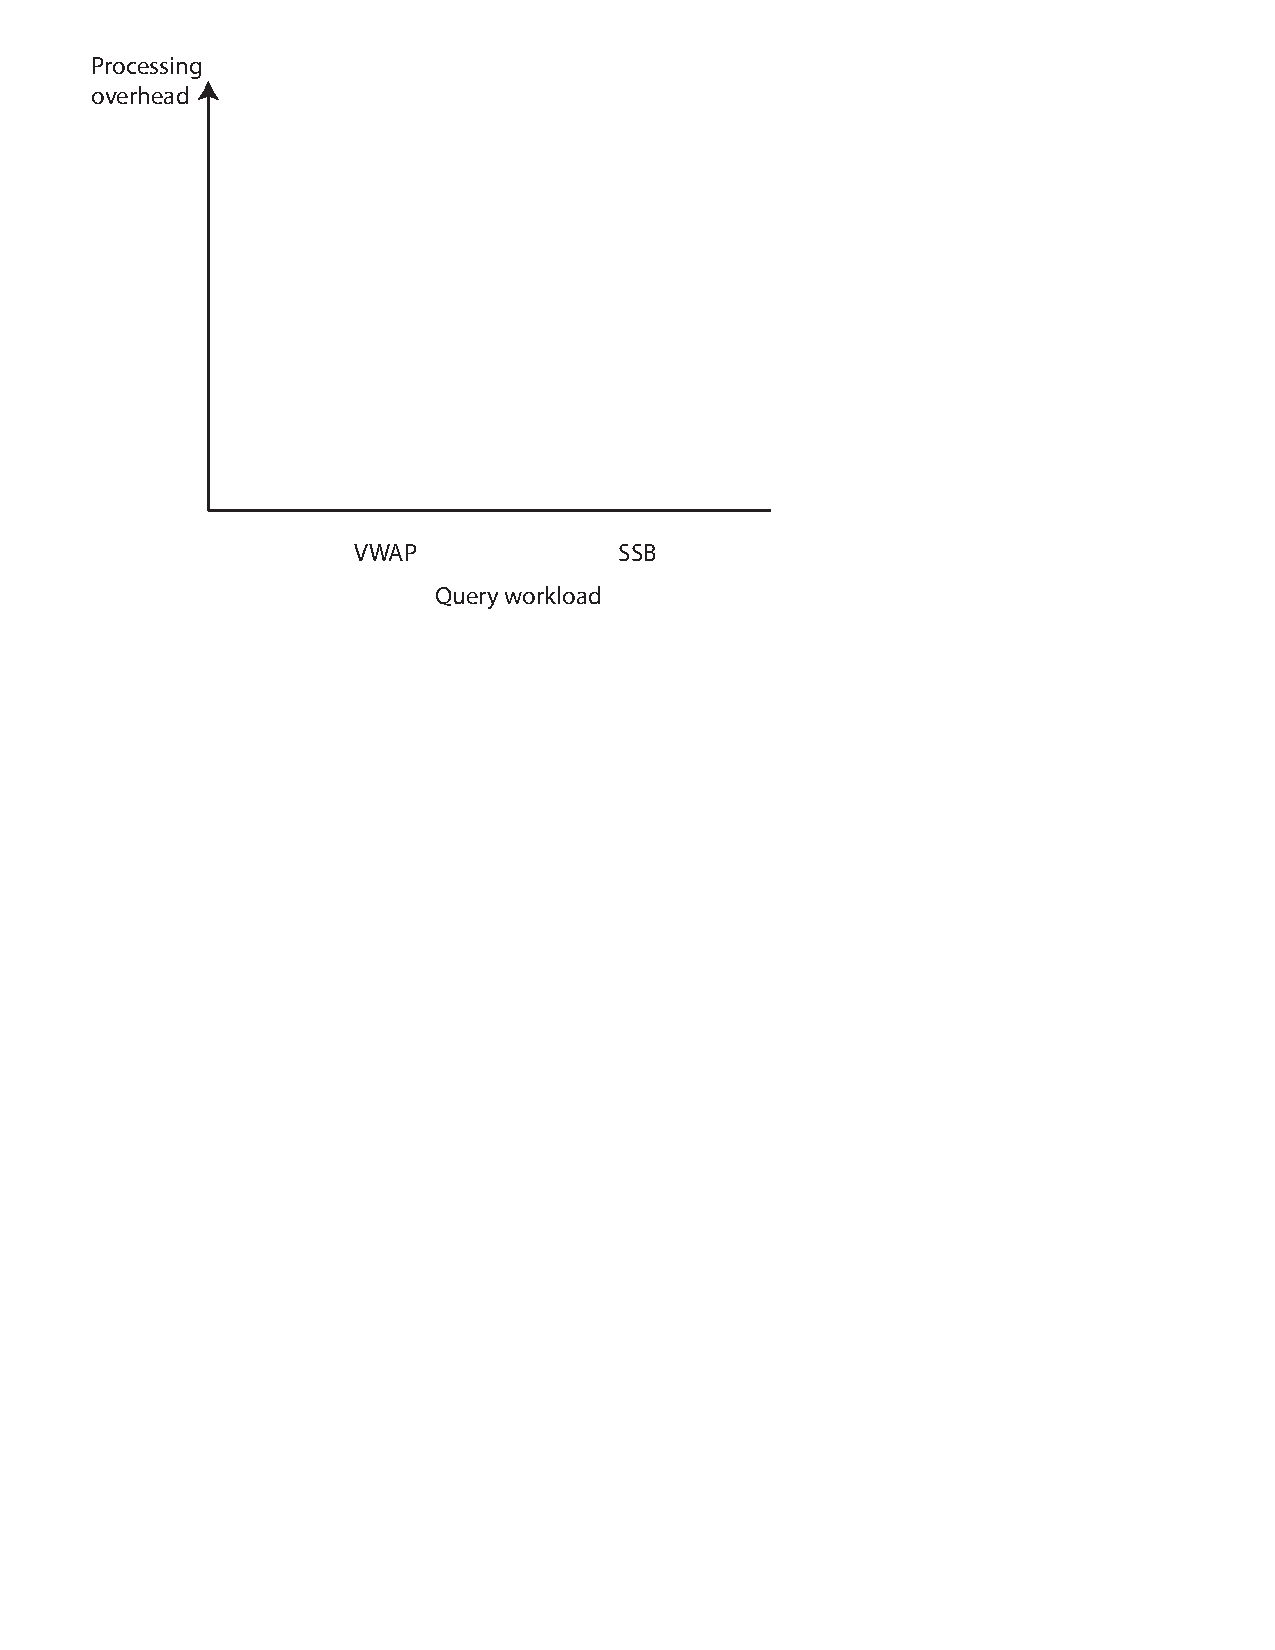
\includegraphics[scale=0.6]{figures/axes-query.pdf}
\caption{Query processing overheads for the VWAP and SSB queries, for naive
  query processing, incremental view maintenance and DBToaster.}
\label{fig:overhead-vwap-ssb}
\end{figure}

\subsection{Memory Utilization}
\begin{itemize}
\item Measure total process memory usage over time, taking samples every $k$
  tuples (find a suitable value of $k$, perhaps 1000?).
\item Use the following formula to estimate a std::map$<>$ memory usage:
\begin{align*}
(sizeof(key) & + sizeof(value) + \\
& sizeof(rb\_tree\_node))*N\\
+ sizeof(rb\_tree)
\end{align*}

\item If time permits, use a custom allocator with an identifier for each map
assigned to use the allocator to track memory usage per map.

\item We have the following formulae for the number of maps created for k-way
joins with specific types of join graphs. These are derived by considering the
combinations of subgraphs of size $i$ (which constitute relations we can
aggregate), with $i = [1 \ldots k-1]$
    \begin{itemize}
    \item Chain: $\sum_{i=1}^{k}{i} = \frac{k(k+1)}{2}$
    \item Star: $(\sum_{i=1}^{k-1}{\binom{k-1}{i}}) + k $
    \item Cycle: $k*\sum_{i=1}^{k-1}{i} = \frac{k^2(k-1)}{2}$
    \end{itemize}

\item Predicted memory utilization:
    \begin{itemize}
    \item VWAP: mem(DBToaster) $>$ mem(VM) $>$ mem(naive) -- due to increased
    map usage, while still needing to maintain full domain. This changes if the base
    relation contains many duplicates, i.e. $|dom(P)| << |bids|$.
    \end{itemize}
\end{itemize}

\begin{figure}
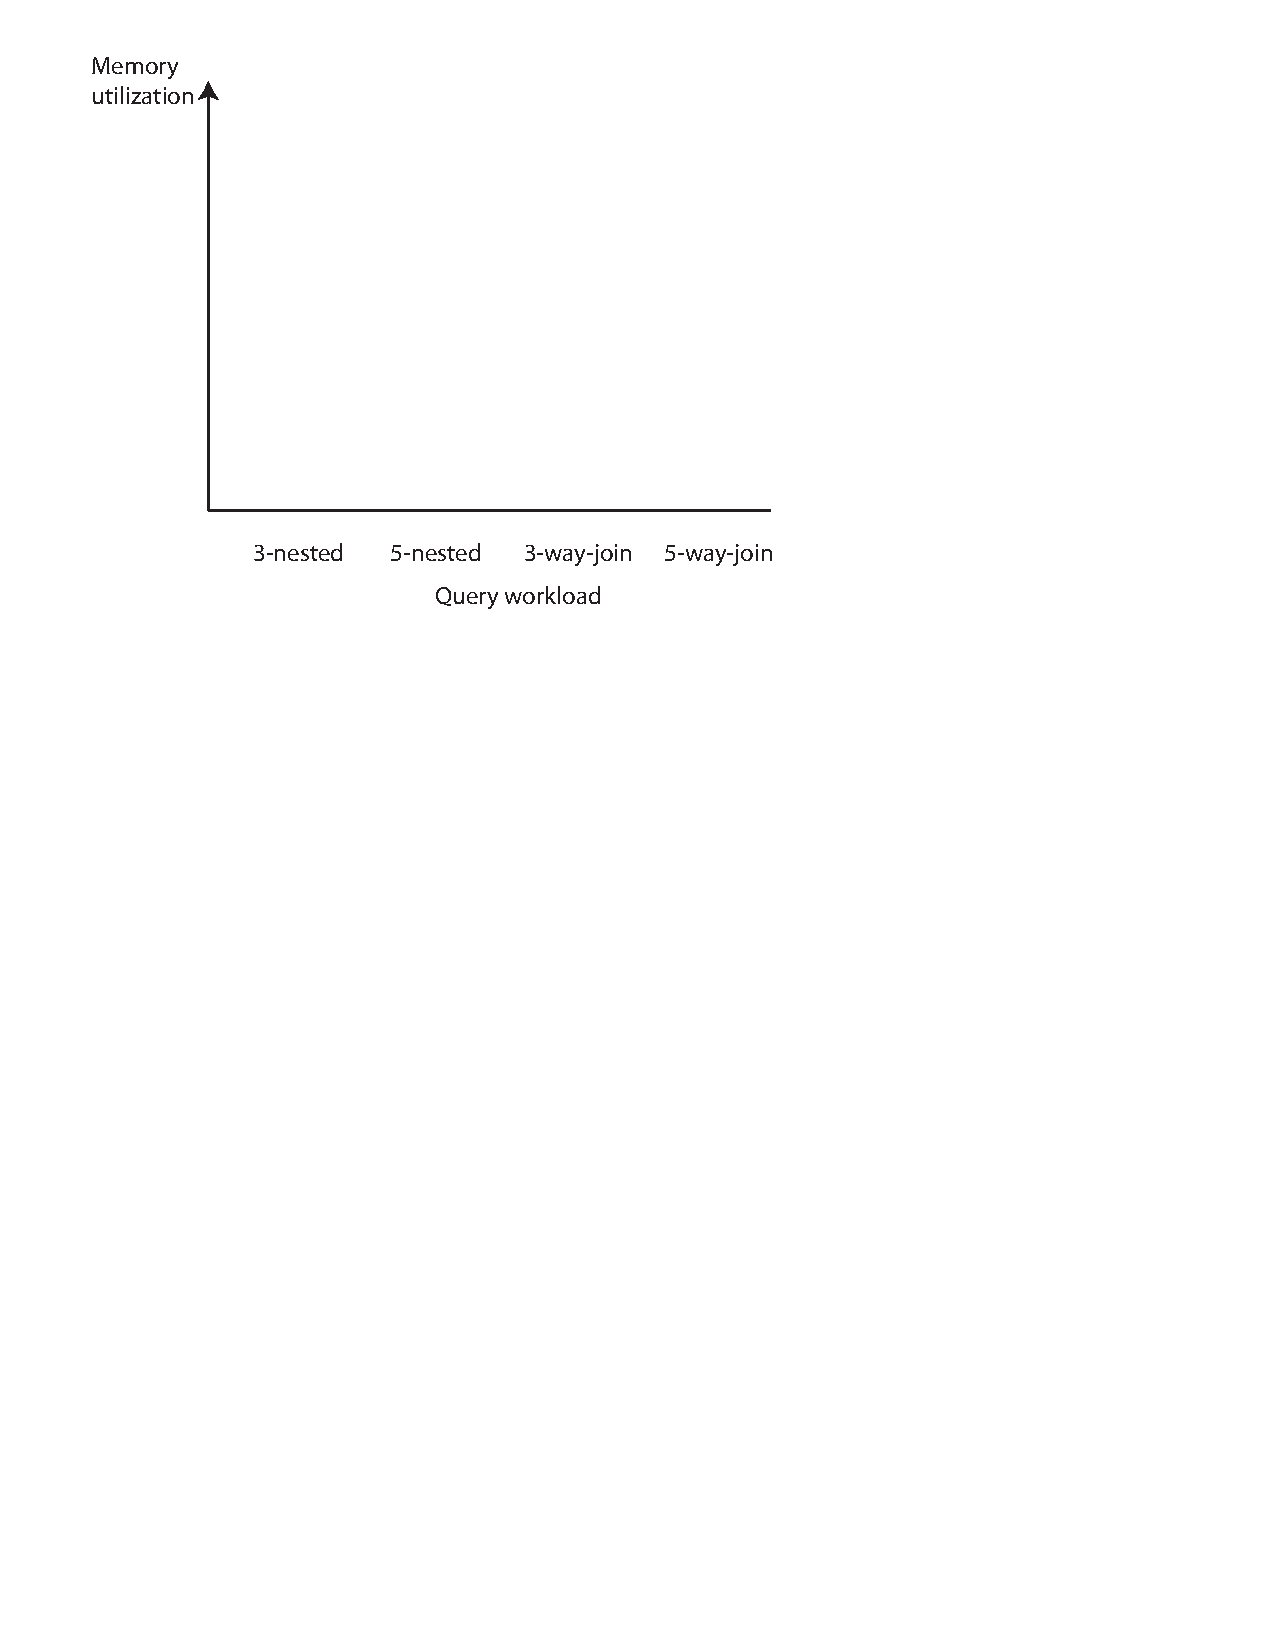
\includegraphics[scale=0.6]{figures/axes-memnjquery.pdf}
\caption{Memory utilization of the naive, incremental view maintenance, and
  DBToaster query processing techniques on nested and multiway join queries.}
\label{fig:memutil-njquery}
\end{figure}

\begin{figure}
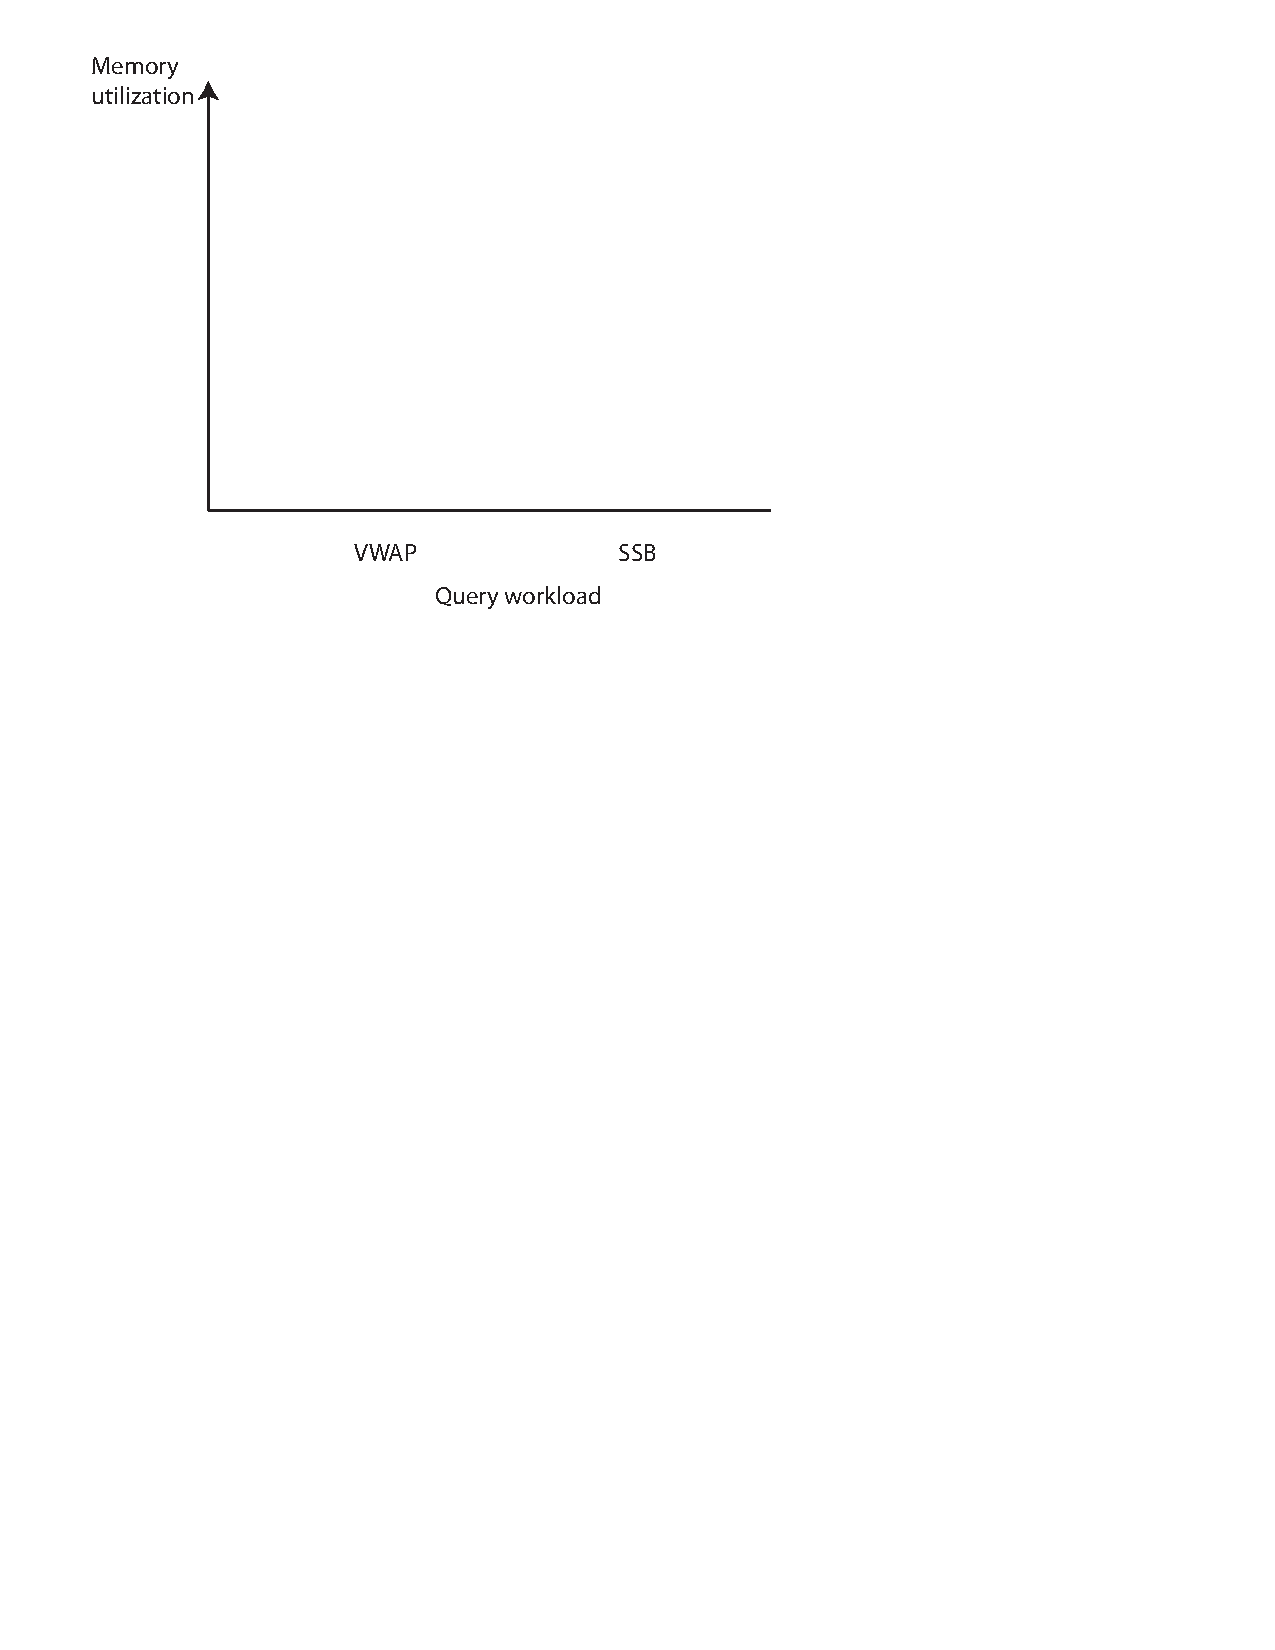
\includegraphics[scale=0.6]{figures/axes-memvsquery.pdf}
\caption{Memory utilization of the naive, incremental view maintenance, and
DBToaster query processing techniques for the VWAP and SSB queries.}
\label{fig:memutil-vsquery}
\end{figure}

\subsection{DBMS Bakeoff}
\begin{itemize}
\item Compare DBToaster to Postgres, HSQLDB, Oracle (DBMS 'X'), Borealis,
  Streambase (DBMS 'Y').
\item Compare using four different techniques: repetitive processing, trigger
  processing, builtin view maintenance, and stream processing.
\item What about a column store, e.g. Vertica/MonetDB? This would only be
  possible under a repetitive QP technique (or does Vertica implement triggers?)
\end{itemize}

\subsubsection{Repetitive Processing}
\begin{itemize}
\item Check whether we can simply pass through queries to Postgres, DBMS 'X' and
  HSQLDB, or whether it's better to generate from map algebra due to specific
  SQL syntax for each DBMS.
\item Run experiment for repeating at various fractions of the dataset size,
  i.e. 10\%,20\%,...,100\%, where 100\% means running the query for every tuple.
\item Note other DBMS can exploit caching here significantly, while DBToaster
  currently does not perform caching, and is L1/L2 cache-agnostic.
\end{itemize}

\begin{figure}
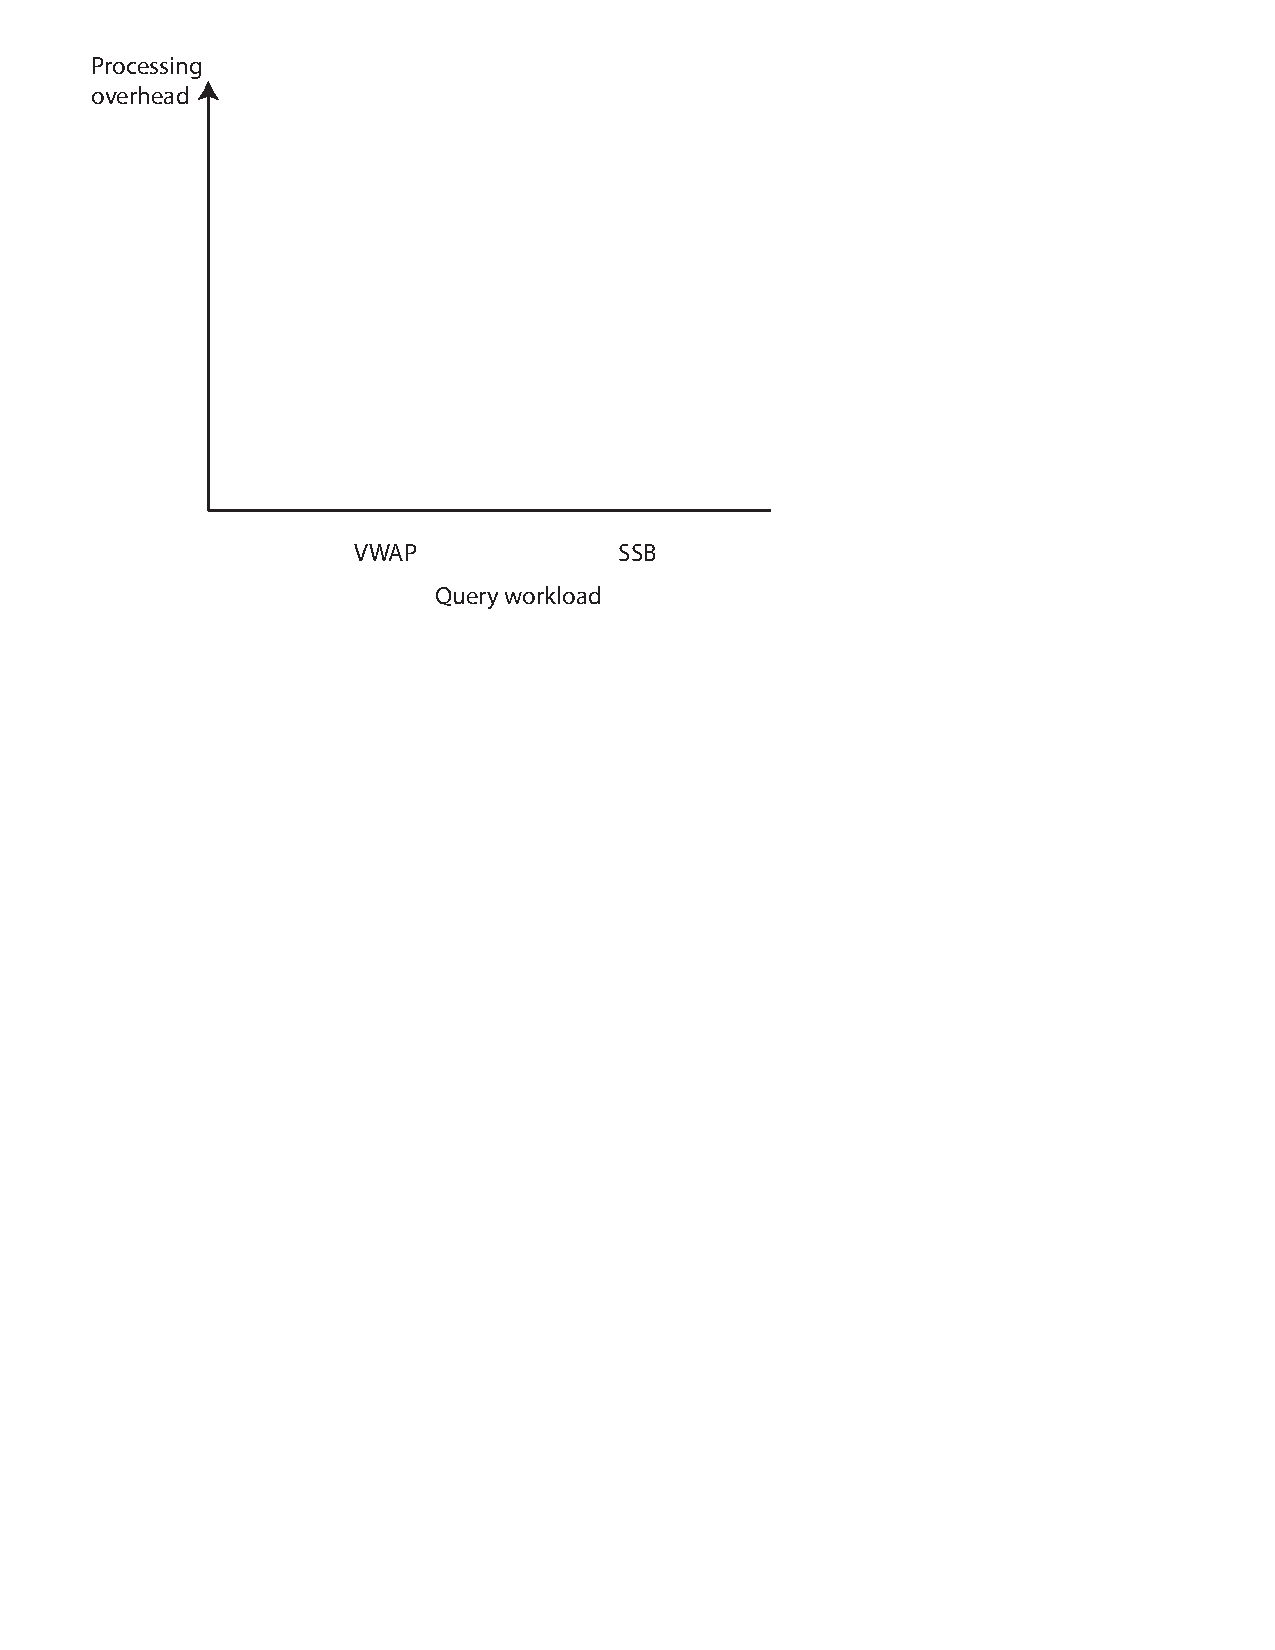
\includegraphics[scale=0.6]{figures/axes-repetitive.pdf}
\caption{Comparison of repetitive ad-hoc query processing of the VWAP and SSB
queries, in Postgres, DBMS 'X' and HSQLDB, to DBToaster's compiled query
processing.}
\label{fig:overhead-repetition}
\end{figure}

\subsubsection{Trigger-based processing}
\begin{itemize}
\item Generate trigger code from map algebra: use temporary tables as maps, and
  generate trigger code corresponding to each handler function.
\item HSQLDB only has Java-based triggers. Let's skip generating such Java-based
  triggers for now.
\item Postgres only allows row-based triggers to inspect tuple contents, DBMS
  'X' may allow access to the old and new tuple sets, allowing set-based
  triggering (like SQL Server).
\end{itemize}

\begin{figure}
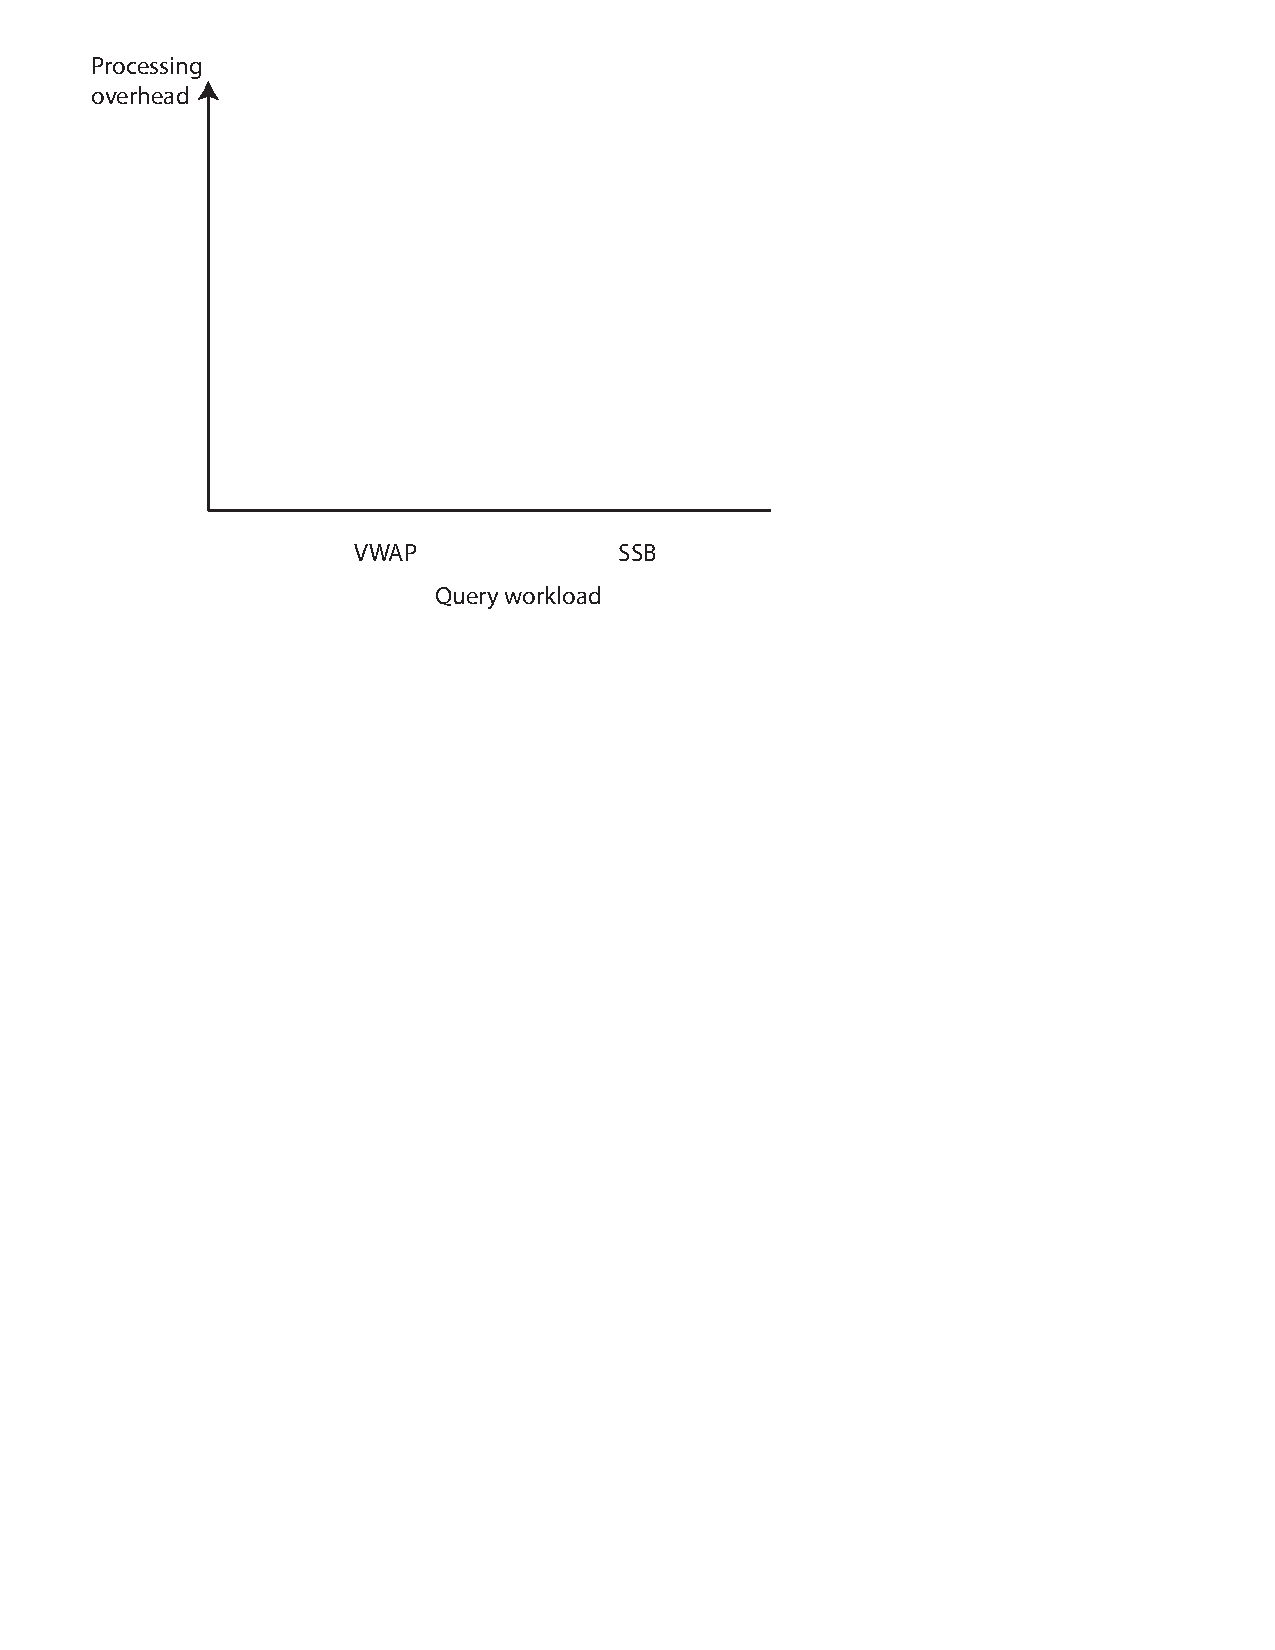
\includegraphics[scale=0.6]{figures/axes-triggers.pdf}
\caption{Comparison of trigger-based processing of the VWAP and SSB queries in
Postgres, DBMS 'X' and HSQLDB to DBToaster's compiled query processing}
\label{fig:overhead-trigger}
\end{figure}

\subsubsection{Materialized view maintenance}
\begin{itemize}
\item Pick a feasible query for view maintenance (perhaps TPCH/SSB queries...) since
  VWAP cannot be done via incremental view maintenance in DBMS 'X'.
\item Check if we can simply pass through user-specified query to DBMS 'X's create
  view DDL statement.
\end{itemize}

\begin{figure}
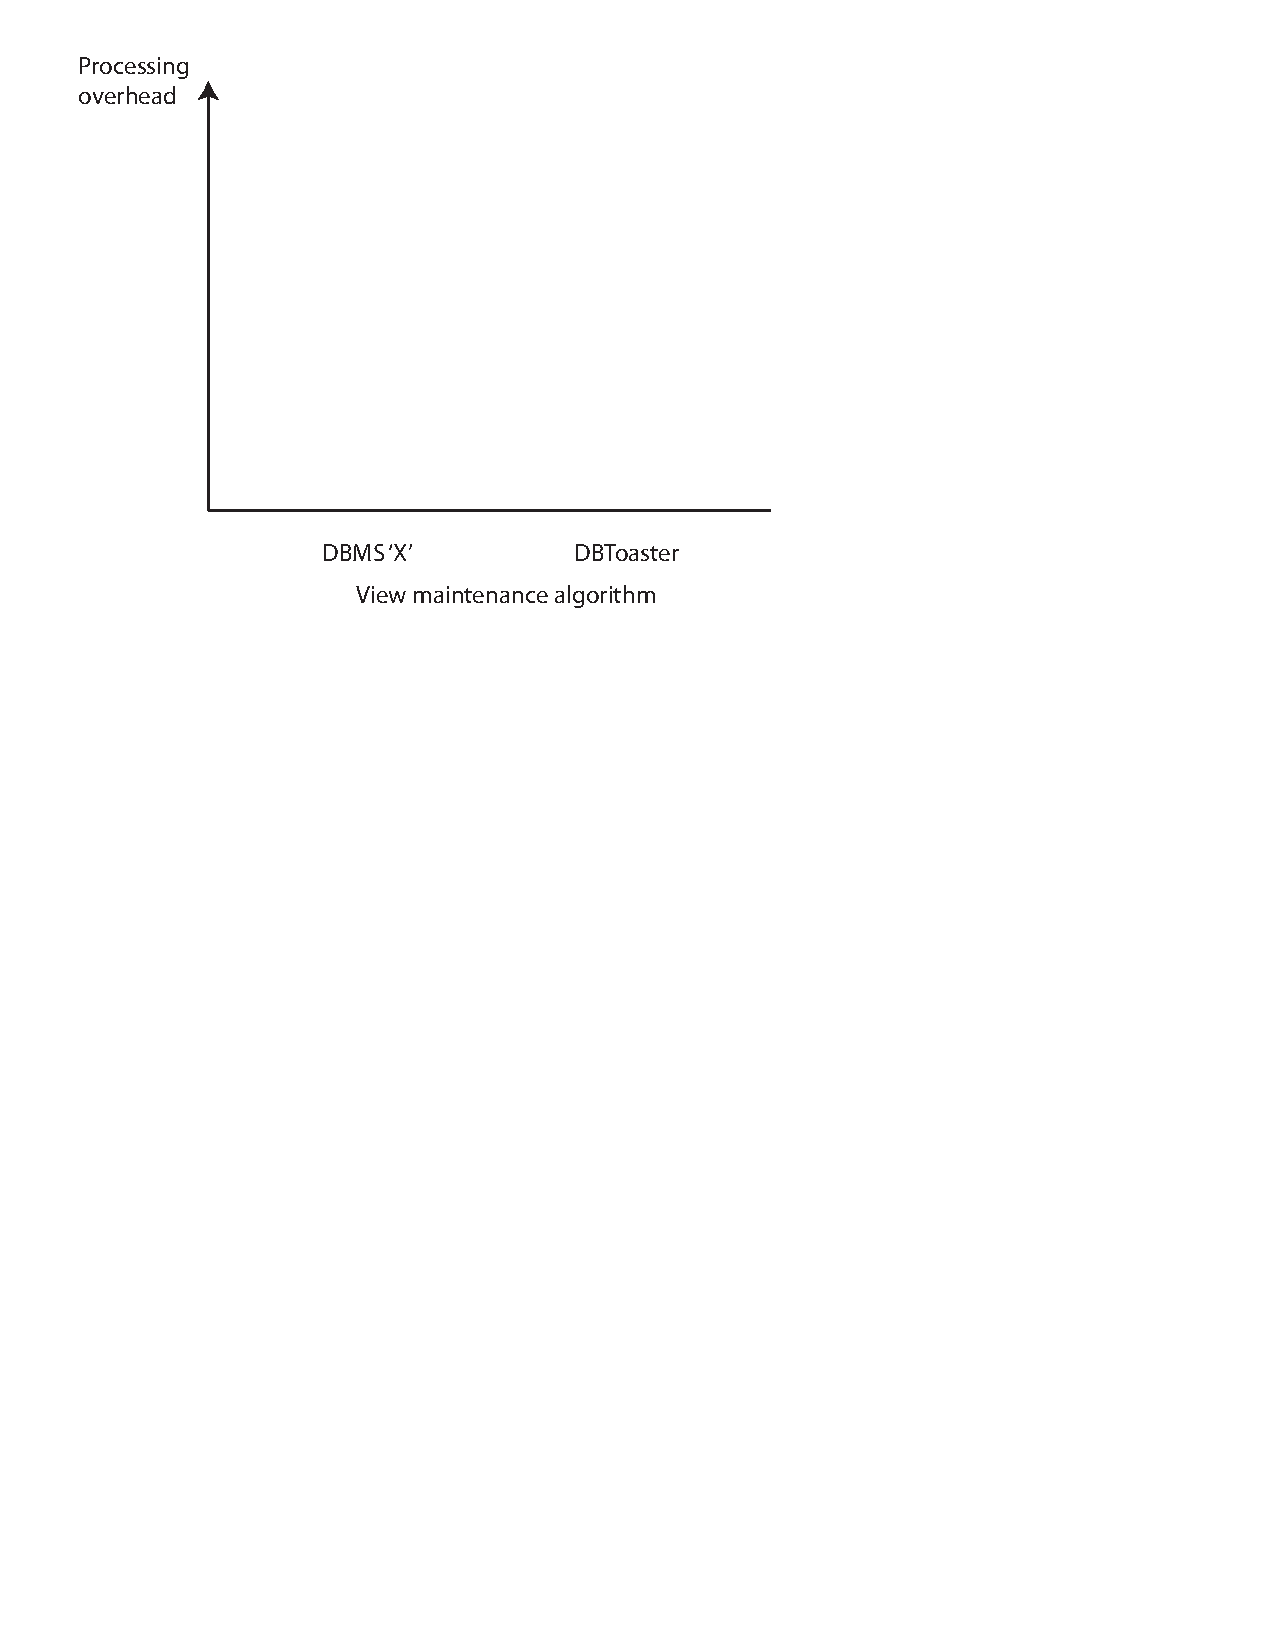
\includegraphics[scale=0.6]{figures/axes-views.pdf}
\caption{Comparison of view maintenance in DBMS 'X' to DBToaster's compiled query processing}
\label{fig:overhead-trigger}
\end{figure}

\subsubsection{Stream processing}
\begin{itemize}
\item Pick a feasible query for stream processing (i.e., pure stream processing
  query, perhaps Linear Road avg lav), that does not require the use of
  in-memory tables.
\item Compare both VWAP query and pure-stream query (i.e. with windowing
  expressed as a range predicate in DBToaster).
\item Generate Borealis XML representation and Streambase app XML representation
  directly from initial map algebra.
\end{itemize}

\begin{figure}
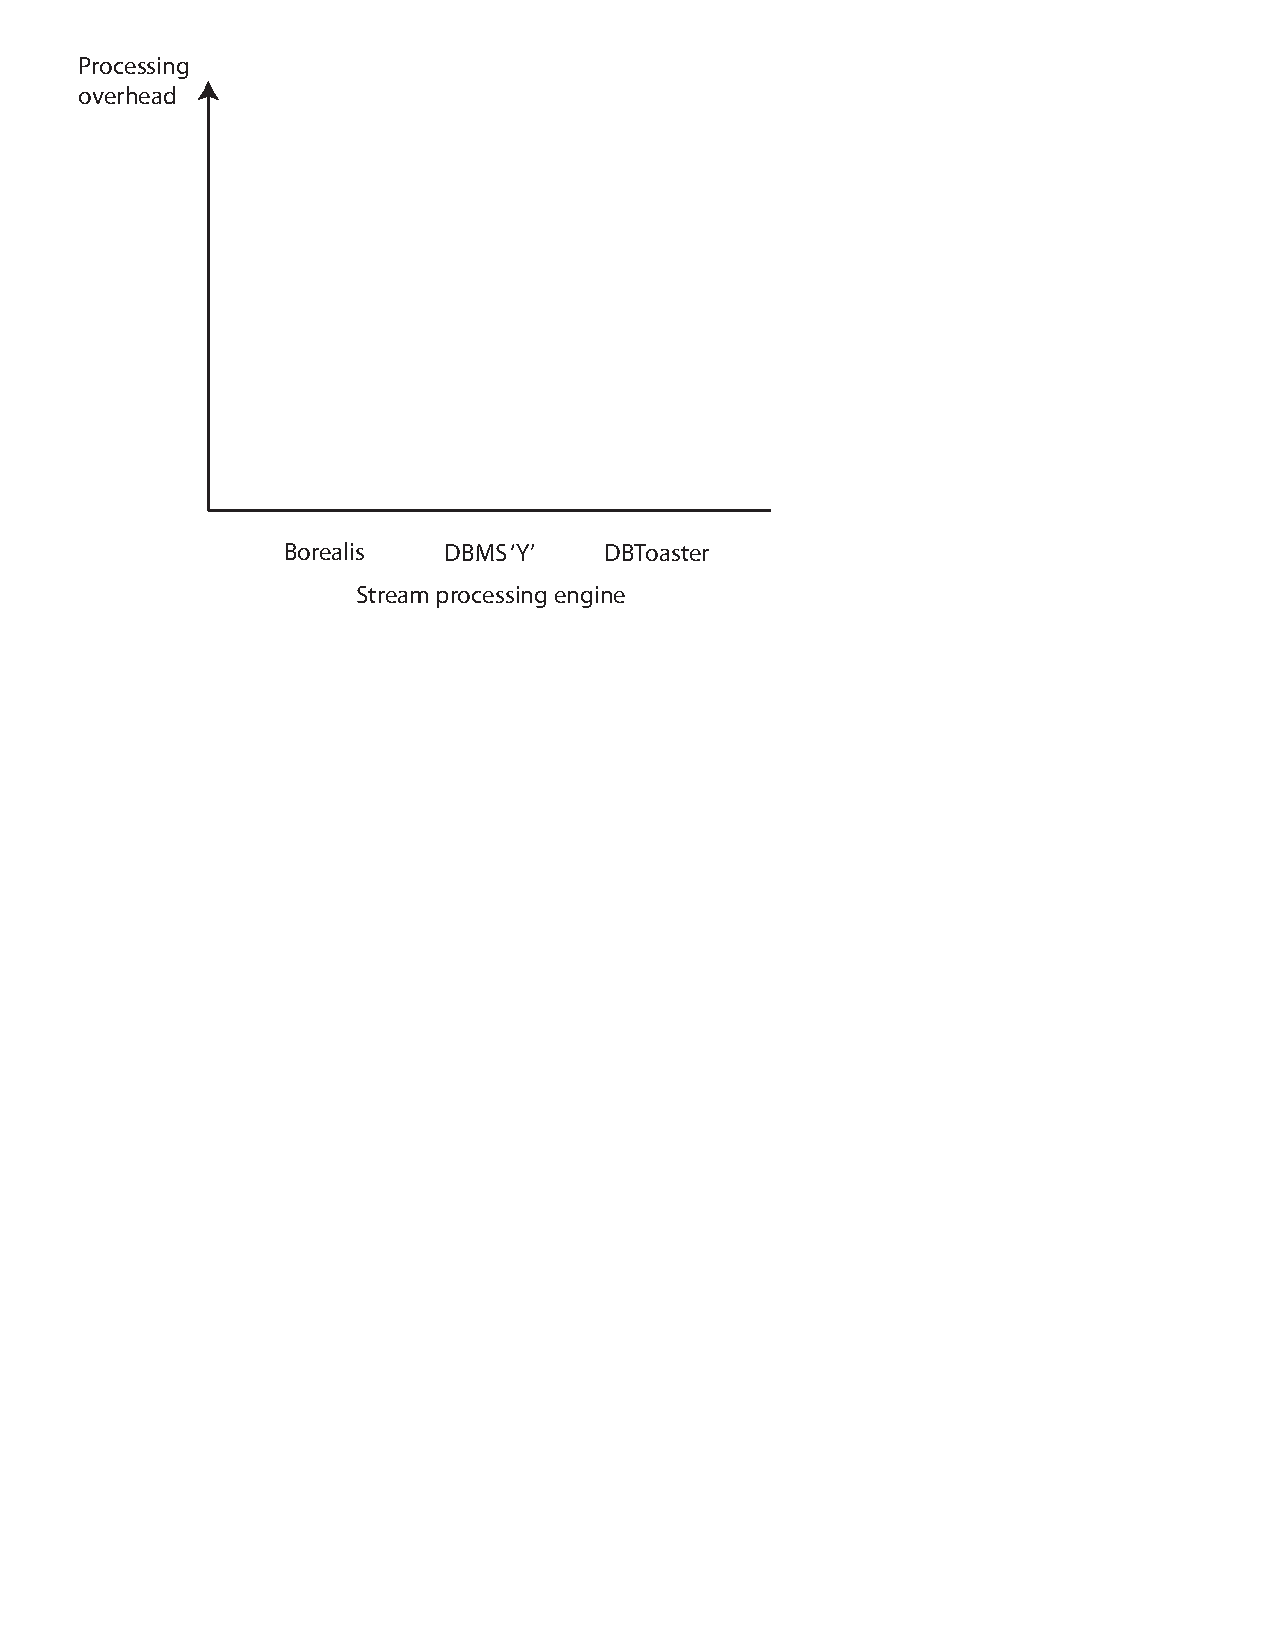
\includegraphics[scale=0.6]{figures/axes-streams.pdf}
\caption{Comparison of stream processing implementations of the XXX query, for
  Borealis and DBMS 'Y' to DBToaster's compiled query processing.}
\label{fig:overhead-stream}
\end{figure}

\subsection{DBToaster Cost Model}

\section{Related Work}

\section{Conclusions}

\end{document}